\chapter{Исследовательский раздел}\label{research}

Вычисляемое значение информационной энтропии разработанным методом подсчета должно коррелировать с показателями качества сжатия, описанными в подразделе \ref{compression-indicators}: коэффициентом сжатия, экономией пространства и силой сжатия. В соответствии с этим проводится исследование корреляции получаемого значения энтропии и указанных характеристик.

Так как на качество сжатия помимо алгоритма сжатия влияет их структура, производится исследование зависимости показателей качества сжатия и времени сжатия от различных типов хранимых в памяти данных.

Для анализа временной эффективности разработанной оптимизации выполняется исследование соотношения времени сжатия и времени вычисления энтропии при записи данных в устройство zram.

Для проведения исследований используются следующие данные:

\begin{itemize}
    \item exec-test.tar --- архив, содержащий исполняемые файлы из директории /usr/bin;
    \item text-test.tar --- архив, состоящий из текстовых файлов исходного кода ядра Linux \cite{linux-code};
    \item pdf-test.tar --- архив, включающий в себя файлы с расширением .pdf из открытого набора резюме livecareer.com \cite{resume-dataset};
    \item img-test.tar --- архив, составленный из файлов с расширением .jpg из открытого набора изображений цветов \cite{flowers-dataset}.
\end{itemize}

\section{Исследование корреляции энтропии и качества сжатия}

На рисунке \ref{img:correlation-matrix} приведена матрица корреляции, составленная с помощью коэффициента корреляции Пирсона. Построенная матрица корреляции устанавливает зависимости между следующими характеристиками:

\begin{itemize}
    \item значением энтропии, вычисляемой разработанным методом подсчета;
    \item значением энтропии, определяемой методом скользящего окна;
    \item значением энтропии, подсчитанной биномиальным методом;
    \item коэффициентом сжатия;
    \item экономией пространства;
    \item силой сжатия.
\end{itemize}

\begin{figure}[H]
	\begin{center}
		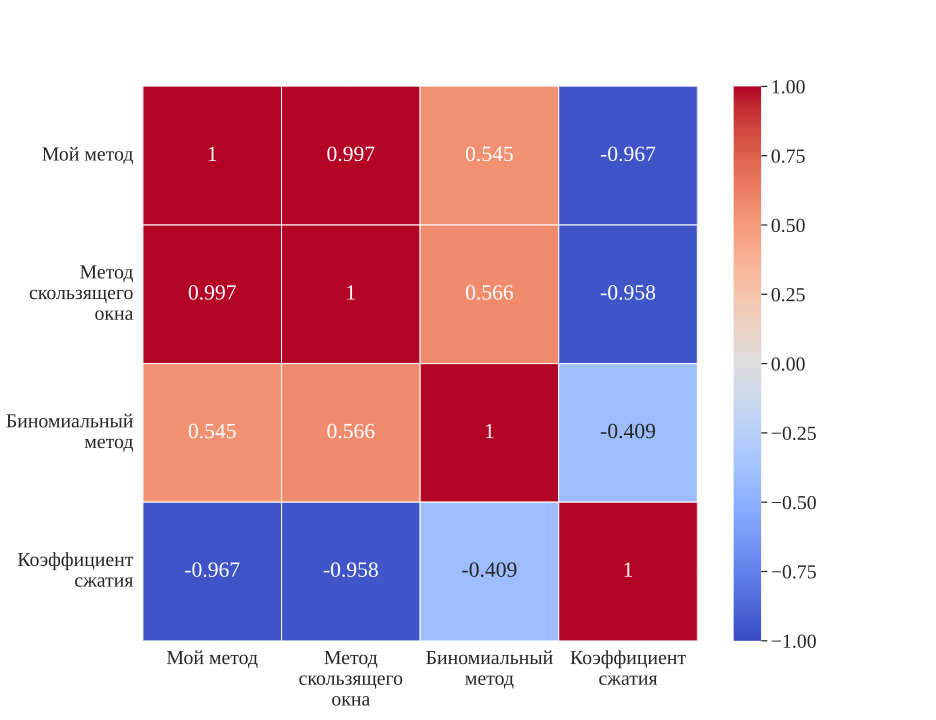
\includegraphics[scale=0.4]{inc/img/correlation-matrix.pdf}
	\end{center}
	\captionsetup{justification=centering}
	\caption{IDEF0-диаграмма первого уровня}
	\label{img:correlation-matrix}
\end{figure}

В результате анализа полученной матрицы корреляции можно сделать следующие выводы:

\begin{enumerate}
    \item Значения энтропии, вычисляемые описанными методами подсчета, обладают высокой отрицательной корреляцией с показателями качества сжатия. При этом корреляция значений энтропии с показателями качества сжатия, определяемых разработанным методом и методом скользящего окна, выше корреляции энтропии, получаемой биномиальным методом.
    \item Значения энтропии, вычисляемые указанными методами подсчета, обладают высокой положительной корреляцией друг с другом.
\end{enumerate}

Так, энтропия, вычисляемая разработанным методом, обладает высокой отрицательной корреляцией с показателями качества сжатия, сравнимой с корреляцией энтропии, определяемой методом скользящего окна, и большей корреляции энтропии, получаемой биномиальным методом.

\section{Исследование зависимости характеристик от типов хранимых в памяти данных}

На рисунках \ref{img:format-ratio}-\ref{img:format-time} представлены зависимости коэффициента сжатия, экономии пространства, силы сжатия и времени сжатия от формата сжимаемых данных алгоритмами сжатия zstd, lz4, lz4hc, lzo и lzo-rle.

\includeimage
    {format-ratio}
    {f}
    {h}
    {1.0\textwidth}
    {Зависимость коэффициента сжатия от формата данных}

\includeimage
    {format-space}
    {f}
    {h}
    {1.0\textwidth}
    {Зависимость экономии пространства от формата данных}

\includeimage
    {format-gain}
    {f}
    {h}
    {1.0\textwidth}
    {Зависимость силы сжатия от формата данных}

\includeimage
    {format-time}
    {f}
    {h}
    {1.0\textwidth}
    {Зависимость времени сжатия от формата данных}

В результате анализа построенных гистограмм можно сделать следующие выводы:

\begin{enumerate}
    \item Наибольшие значения показателей качества сжатия у текстовых данных.
    \item Значения показателей качества сжатия у исполняемых файлов меньше, чем у текстовых, но больше, чем у PDF-файлов.
    \item Наименьшие значения показателей качества сжатия у изображений.
    \item Наибольшее время сжатия у исполняемых файлов.
    \item Время сжатия текстовых данных меньше, чем у исполняемых, но больше, чем у PDF-файлов.
    \item Наименьшее время сжатия у изображений.
\end{enumerate}

Данные с расширениями .pdf и .jpg являются сжатыми данными, поэтому значения показателей качества для указанных данных меньше, чем для текстовых и исполняемых данных.

\section{Исследование временной эффективности}

В таблице \ref{tab:time-efficiency} показано соотношение времени сжатия и времени вычисления информационной энтропии для доступных в модулей zram алгоритмов сжатия: zstd, lz4, lz4hc, lzo и lzo-rle. Столбчатые диаграммы, соответствующие полученным результатам, приведены на рисунке \ref{img:time-efficiency}.

\begin{table}[h]
    \caption{Соотношение времени сжатия и времени вычисления энтропии}
    \begin{center}
        \begin{tabular}{|l|l|l|l|}
                \hline
            \multicolumn{1}{|c}{\textbf{Алгоритм}} & 
            \multicolumn{1}{|c|}{\textbf{Сжатие, \%}} &
            \multicolumn{1}{c|}{\textbf{Вычисление}} &
            \multicolumn{1}{c|}{\textbf{Другие}} \\
            \multicolumn{1}{|c}{\textbf{сжатия}} & 
            \multicolumn{1}{|c|}{\textbf{}} &
            \multicolumn{1}{c|}{\textbf{энтропии, \%}} &
            \multicolumn{1}{c|}{\textbf{функции, \%}} \\ \hline
            zstd & 84 & 12 & 4 \\ \hline
            lz4 & 58 & 32 & 10 \\ \hline
            lz4hc & 89 & 8 & 3 \\ \hline
            lzo & 61 & 31 & 8 \\ \hline
            lzo-rle & 60 & 31 & 9 \\ \hline
        \end{tabular}
    \end{center}
    \label{tab:time-efficiency}
\end{table}

\includeimage
    {time-efficiency}
    {f}
    {h}
    {0.6\textwidth}
    {Соотношение времени сжатия и времени вычисления энтропии}

В результате анализа построенных гистограмм можно сделать следующие выводы:

\begin{enumerate}
    \item Время вычисления энтропии в семь раз меньше времени сжатия страниц для алгоритма сжатия zstd.
    \item Время вычисления энтропии почти в 1.81 раз меньше времени сжатия страниц для алгоритма сжатия lz4.
    \item Время вычисления энтропии в 11.13 раз меньше времени сжатия страниц для алгоритма сжатия lz4hc.
    \item Время вычисления энтропии в 1.97 раз меньше времени сжатия страниц для алгоритма сжатия lzo.
    \item Время вычисления энтропии в 1.94 раз меньше времени сжатия страниц для алгоритма сжатия lzo-rle.
\end{enumerate}

Таким образом, время вычисления энтропии значительно ниже времени сжатия данных.

\section*{Вывод}

В данном разделе было проведено исследование корреляции показателей качества сжатия и значений информационной энтропии, вычисляемых разработанным методом, методом скользящего окна и биномиальным методом. Построенная с использованием коэффициента Пирсона матрица корреляции показала, что определяемое значение энтропии обладает высокой отрицательной корреляцией с показателями качества сжатия, поэтому может использоваться для оценки качества сжатия.

Была установлена зависимость показателей качества сжатия от типов хранимых в памяти данных: для PDF-файлов и jpg-файлов, которые являются сжатыми данными, характеристики сжатия ниже, чем их значения для текстовых и исполняемых данных.

В результате анализа временной эффективности было выявлено, что время вычисления энтропии значительно ниже времени сжатия. Таким образом, разработанная оптимизация позволяет увеличить скорость обработки несжимаемых страниц памяти в модуле сжатия zram и производительность всей системы в целом.
